%
% Latex example file for postgrads (04/10/03)
%
% If you have questions please email me: 
%
% M.L.Balogh@durham.ac.uk
%
% or find me in room OC312.
%
% you can copy this file and others from :
%
% http://star-www.dur.ac.uk/~balogh/latex/
%
% Note you can get Latex style files etc. from http://www.ctan.org

% Latex2e style  declaration


% The emulateapj.cls file produces output like that of the
% Astrophysical Journal.  Use instead of aastex.cls.  This usage
% supercedes older versions that used the aastex package with emulateapj5.sty.
% YOU SHOULD REMOVE THE TABLE OF
% CONTENTS PAGE WHEN USING APJ FORMAT.
%
\documentclass[11pt,a4paper]{emulateapj}
\bibliographystyle{apj}


%define general packages
\usepackage{epsfig}
\usepackage{amsmath}
\usepackage{natbib}

%internal short cuts
\def \HgA {H$\gamma_A$}
\def \gon {Gonz\'{a}lez}
\def \Hbp {H$\beta ^\prime$}

\begin{document}

\title{COMPLETE View of the Ophiuchus Cloud I: Stellar Wind Driven by B-type Stars}
\author{Hope Chen \& Aaron Meisner}
\date{\today}
%\maketitle


% Usually omit these for ApJ or MNRAS style files:
%\tableofcontents
%
%\listoffigures
%
%\listoftables

\begin{abstract}
\textbf{Abstract} Using data from the COordinated Molecular Probe Line
Extinction Thermal Emission (COMPLETE) Survey of Star Forming Regions
and the complementary data from the Herschel Gould Belt Survey, we
present an analysis of three different column density tracers --
near-infrared extinction, far-infrared dust thermal emission, and
molecular line emission of the \textsuperscript{12}CO J=1-0 and
\textsuperscript{13}CO J=1-0 transitions. In this paper, we compare
column densities based on these three different tracers and try to
provide a prescription for tracing material in various parts of a
molecular cloud. Based on the derived column density and temperature, we
report a shell-like structure that is potentially the result of an
embedded B-star wind. We also examine the variation of the column
density probability distribution function (PDF) across the Ophiuchus
cloud. This is further compared with the information of the cloud
dynamics derived from the \textsuperscript{12}CO and
\textsuperscript{13}CO data. We conclude that one needs to take extreme
care when tracing the column density structure and interpreting its
relation with the dynamics in a molecular cloud. A detailed simulation
with proper synthetic observation is required to explain the
(non-)correlation between the column density PDF and the turbulence
(represented by the Mach number) in the Ophiuchus cloud.

\end{abstract}

%Section heading
\section{Introduction}
\label{sec:introduction}
Nearby Gould Belt Clouds are often targets of star formation observations. Their small distances from the Earth provide astronomers a chance to resolve the star formation activities. The first step to understand the environment of star formation in these clouds is to trace their mass structures. To do so, people often employ three different kinds of methods: molecular line emission, extinction of background stars by the dust in the clouds, and the dust thermal emission in the mid/far-infrared wavelengths.
The first observation of molecular line emission from star forming regions dates back to [????] (Ref?). Observation of line emission provides information of the line-of-sight velocity.
The extinction of background stars corresponds to the amount of dust material 

\section{Data}
\label{sec:data}
In this paper, we use data from the COordinated Molecular Probe Line Extinction Thermal Emission (COMPLETE) Survey of Star Forming Regions. Together with data from a broader collaboration, these include 1) an extinction map based on near-infrared data from the Two Micron All-Sky Survey (2MASS) and a near-infrared color excess method, the NICEST algorithm \citep[][note that this is an improved version of the NICER algorithm and is developed after the COMPLETE Survey]{Lombardi_2009}, 2) 60 and 100 $\mu$m maps from the Improved Reprocessing of the IRAS data \citep[IRIS;]{Miville_Deschenes_2005}, and 3) the molecular line emission of the $^{12}$CO J=1-0 and $^{13}$CO J=1-0 transitions obtained at the Five College Radio Astronomy Observatory (FCRAO). We also include archival Herschel data, which were taken as part of the Herschel Gould Belt Survey. The Herschel data allow us to derive column density and other physical properties based on the more complete SED of far-infrared dust thermal emission than the 60 and 100 $\mu$m bands of the IRIS data.

\subsection{2MASS/NICEST Extinction}
The NICEST algorithm is the latest version of a near-infrared color excess method to derive the dust extinction based on near-infrared observation. Its predecessors include the NICE and the NICER algorithms \citep{Lombardi_2001,Lombardi_2005}.

\subsection{IRAS/IRIS 60 and 100 $\mu$m maps}
The Infrared Astronomical Satellite (IRAS) performed a survey that covered 98 \% of the sky at four wavelenths: 12, 25, 60, and 100 $\mu$m \citep{Neugebauer_1984}. However, the widely used dataset released in 1994 (IRAS Sky Survey Atlas; Wheelock and Infrared Processing and Analysis Center, 1994) suffers from the calibration, zero level, and striping problems. The Improved Reprocessing of the IRAS data \citep[IRIS;]{Miville_Deschenes_2005} provides a significant improvement over these problems. For the purpose of this paper, we use only the 60 and 100 $\mu$m maps of the Ophiuchus region from the IRIS data product and a simple two-band method similar to that used by \citet{Schnee_2008} to derive the column density for the Perseus molecular cloud (see the next section).

\begin{figure*}[ht]
\centering
%% The 'scale' parameter below allows you to scale the figure so that it fits within the page. In this case the figure was scaled to 20% of its original size. Note: for .png files one has to use pdflatex, not classic latex
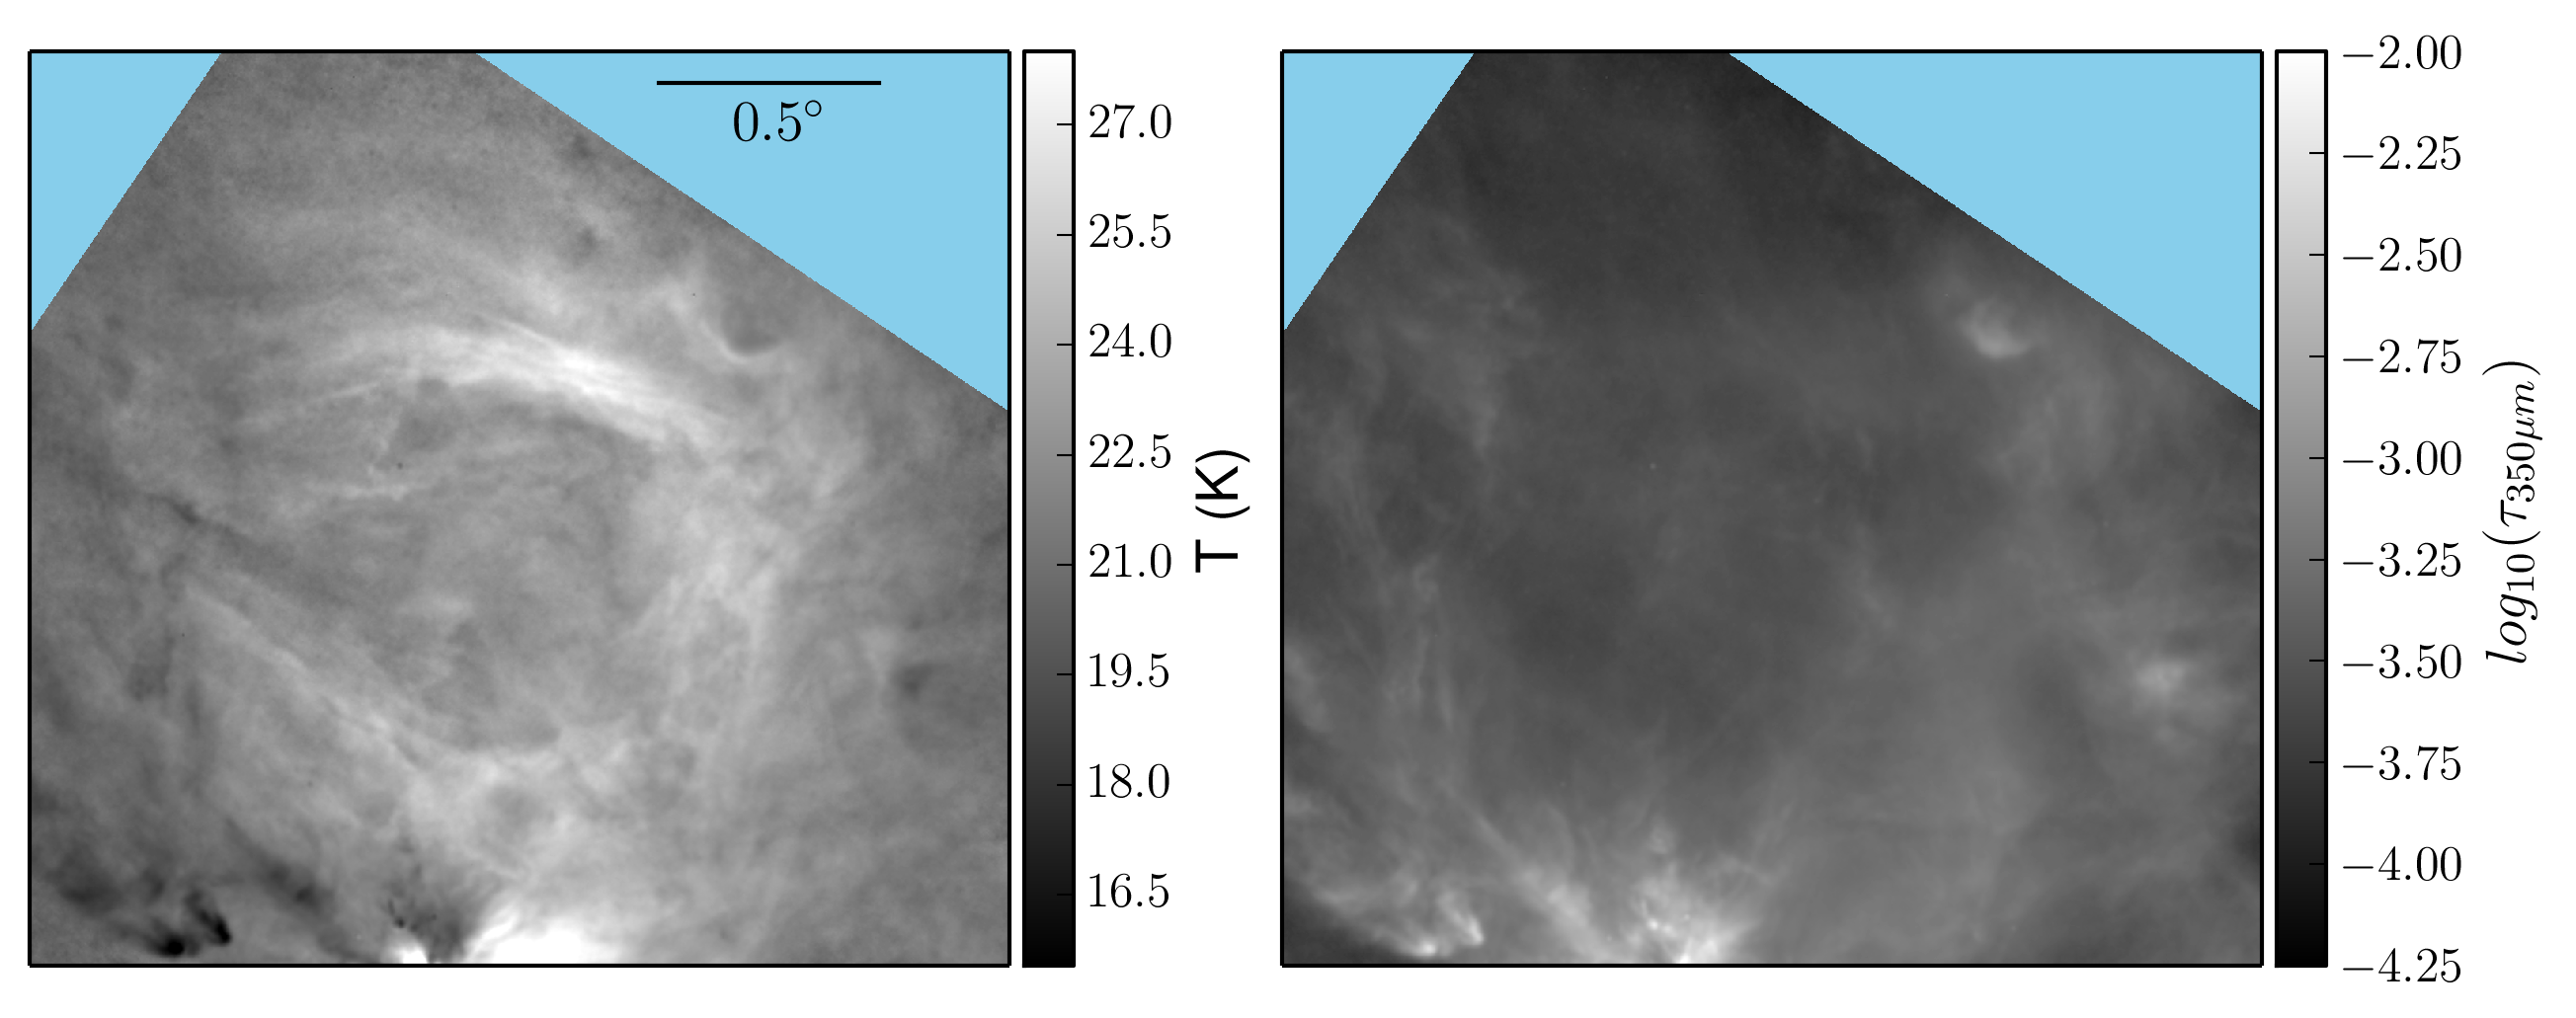
\includegraphics[scale=0.8]{fig/shell_herschel.png}
\caption{The image shows \textit{Herschel}-based temperature and opacity at 350 $\mu$m.
}
\end{figure*}

\subsection{Herschel Archival Data}
The Herschel Space Observatory was a satellite operated by the European Space Agency. Its Photodetecting Array Camera and Spectrometer (PACS) and Spectral and Photometric Imaging Receiver (SPIRE) covered wavelengths from 55 to 670 $\mu$m, with six wide spectral bands: 70, 100, and 160 $\mu$m bands of PACS and 250, 350, and 500 $\mu$m bands of SPIRE. A wide range of the Herschel data products is availabel in the Herschel Science Archive. In this paper, we use data that were obtained as part of the Herschel Gould Belt Survey \citep{Andr__2010}. The maps presented in this paper are produced in the Herschel Interactive Processing Environment (HIPE; Version 11.1.0 was used to produce these maps). The zero level problem is resolved by comparing the maps with predictions from the two-component dust model fitted to the Planck HFI maps of the Ophiuchus region (Meisner \& Finkbeiner, submitted; ArXiv:1410.7523). Again, for the purpose of this paper, only maps of the longest four wavelengths (160 $\mu$m of PACS and 250/350/500 $\mu$m of SPIRE) are used here, since emission at wavelengths shorter than 100 $\mu$m shows significant contribution from emission of ``very small grains (VSGs)'' and requires a dust model more complicated than described by Meisner \& Finkbeiner (submitted). The same situation applies to the IRIS 60 and 100 $\mu$m maps, and an estimate of error is given by \citet{Schnee_2006} and \citet{Schnee_2007}.

\subsection{Molecular Line Emission: $^{12}$CO (1-0) and $^{13}$CO (1-0)}
Observations of molecular line emission of the $^{12}$CO J=1-0 and $^{13}$CO J=1-0 transitions were carried out at the 14m Five College Radio Astronomy Observatory \citep[FCRAO;]{Ridge_2006}. The SEQUOIA 32-element focal-plane array was used to make an on-the-fly map of the Ophiuchus region. A total bandwidth of 25 MHz with 1024 channels in each IF in the dual-IF mode yielded an effective velocity resolution of 0.07 km s$^{-1}$. This allows us to resolve subsonic velocity structures in a typical molecular cloud environment \citep[with a temperature of 15 K and an average molecular weight of 2.33 m$_H$;]{Carey_1998,Pillai_2006}.

\section{Methods}
\label{sec:methods}
Figure 1 shows the column densities based on the data described in Section \ref{sec:data}. For comparison, column densities are converted to the unit of V-band extinction (A$_V$) using a uniform conversion factor of N(H$_2$)/A$_V$ = 6.9 $\times$ 10$^{20}$ cm$^{-2}$ mag$^{-1}$ \citep{Draine_2003,Evans_2009}. (Different factors were suggested for more diffuse regions, for example, N(H$_2$)/A$_V$ = 9.4 $\times$ 10$^{20}$ cm$^{-2}$ mag$^{-1}$ by \citet{Bohlin_1978}.) For the 2MASS/NICEST extinction map, we assume a linear reddening law of A$_K$/A$_V$ = 0.114. Besides the column density, other physical properties including the temperature are derived from these data based on respective assumptions described as follows.

\subsection{Modeling far-infrared emission with a single-component modified blackbody equation}
For both the IRIS and the Herschel data, we assume that the emission at respective wavelengths (60 and 100 $\mu$m for the IRIS maps, and 160/250/350/500 $\mu$m for the Herschel PACS and SPIRE maps) is dominated by the ``big grain \citep[BG;]{Stepnik_2003}'' dust thermal emssion. We also assume that the dust thermal emission can be described by a single-component modified blackbody equation. This assumption is true only on certain conditions and can be a very coarse approximation at wavelengths shorter than 100 $\mu$m. This is because that the emission at wavelengths shorter than 100 $\mu$m starts to see ``contamination'' from the VSG emission. \citet{Schnee_2007} examined this effect and gave an estimate of error for a similar method to derive the column density and dust temperature. They conluded that the typical error at 60 $\mu$m is around 20\% and smaller for longer wavelengths. Since our goal here is to provide a a relative comparison of the IRIS and the Herschel data, using maps of emission at the longest two of the IRAS wavelengths suffices.


\subsubsection{Temperature and column density from the Herschel data}
Similarly, we assume that the emission at Herschel PACS 160 $\mu$m and SPIRE 250/350/500 $\mu$m bands is dominated by the dust thermal emission and can be described by a single modified blackbody equation. This is a better assumption for the Herschel data used in this paper, since the VSG emission shows up mostly at wavelengths shorter than 100 $\mu$m.

\subsubsection{Modeling far-infrared emission with a single-component modified blackbody equation}
Using a single-component modified blackbody equation presumes that the material along the line of sight has a single temperature.

Finally, as \citet{Finkbeiner_1999} and Meisner \& Finkbeiner (submitted; ArXiv:1410.7523) suggested, the modeling is improved by using a two-compoenent modified blackbody equation with a ``hot dust component'' and a ``cold dust component.'' The emission is then described by the equation:

By comparing the two-component model to the single-component model, Meisner \& Finkbeiner (submitted) found that the single-component modified blackbody equation generally underpredicts dust emission at all Planck spectral bands from 100 to 3000 GHz (2 mm to 67 $\mu$m). This is consistent with our analysis above.

Although the wavelength range suggested by Meisner \& Finkbeiner where one should adopt the two-component model covers the two IRAS wavelengths (60 and 100 $\mu$m) and the four Herschel wavelengths (160, 250, 350, and 500 $\mu$m) conisdered in this paper, we use a single modified blackbody equation in consistency with works done by the Gould Belt Survey team. Analysis of the two-component model is beyond the scope of this paper.

\subsubsection{Temperature-spectral index anti-correlation and a Bayesian solution}

\citet{Kelly_2012} suggested a solution to the artificial anti-correlation between the temperature and the spectral index, using a hierarchical Bayesian method.

However, the hierarchical Bayesian method is highly computation-expensive. Assuming a linear law between the computation time and the number of pixels on the map, we estimate the total computation time of one month to finish the calculation of the column density and temperature using the hierarchical Bayesian method, for a map as large as the Herschel maps of the Ophiuchus cloud in Figure 1.

\subsubsection{FCRAO Molecular Line Emission}
We follow the analysis in \citet{Pineda_2008} to derive the equivalent V-band extinction from the $^{12}$CO (1-0) and $^{13}$CO (1-0) line observations. We start by assuming that the $^{12}CO$ is optically thick. We then calculate the excitation temperature using the main beam temperature at the peak of $^{12}CO$:

\begin{equation}
T_{\text{ex}} = \frac{5.5\,\text{[K]}}{\ln{\left(1+5.5\,\text{[K]}/\left(T_{\text{max}}(^{12}\text{CO})+0.82\,\text{[K]}\right)\right)}}\;\;\;\text{,}
\end{equation}

where $T_{\text{max}}(^{12}\text{CO})$ is the brightness temperature at the peak. If the excitation temperature of the $^{13}CO$ (1-0) line is the same as the $^{12}CO$ (1-0), we can calculate the optical depth of the $^{13}CO$ (1-0) line:

\begin{equation}
\tau(^{13}\text{CO}) = - \ln\left[1 - \frac{T_{\text{max}}(^{13}\text{CO})/5.3\,\text{[K]}}{1/\left(e^{5.3\,\text{[K]}/T_{\text{ex}}}-1\right) - 0.16}\right]
\end{equation}

Similarly, here $T_{\text{max}}(^{12}\text{CO})$ is the main beam brightness temperature at the peak of $^{13}CO$. Using the definition of column density in Rohlfs \& Wilson (1996), we can derive the $^{13}CO$ column density from the two equations above:

\begin{equation}
N(^{13}\text{CO}) = 3.0\times10^{14}\;\left[\frac{\tau(^{13}\text{CO})}{1-e^{-\tau(^{13}\text{CO})}}\right]\,\frac{W(^{13}\text{CO})}{1-e^{-5.3\,\text{[K]}/T_{\text{ex}}}}\;\text{[cm}^{-2}\text{]}\;\;\;\text{,}
\end{equation}

where $W(^{13}\text{CO})$ is the integrated intensity along the line of sight in units of [K km/s]. Similarly, we then fit the conversion from both $N(^{13}\text{CO})$ and $W(^{13}\text{CO})$ to the 2MASS extinction.

\begin{equation}
\begin{aligned}
A_V &= X_{N(^{13}\text{CO})}\,N(^{13}\text{CO}) \\
A_V &= X_{W(^{13}\text{CO})}\,W(^{13}\text{CO})
\end{aligned}
\end{equation}

\subsection{Column density probability distribution function (PDF)}


\section{Results}
\label{sec:results}

\subsection{Energy/Momentum Estimation}
To estimate the contribution of the embedded B-star wind to the turbulence in the Ophiuchus, we adopt the near-infrared extinction for the mass calculation (reasons discussed above in \S4.1) and the molecular line emission for the velocity calculation. The molecular line emission provides the resolution as well as the dispersion along the velocity axis. Thus, we base our calculation on the 2MASS extinction map and the FCRAO $^{12}$CO/$^{13}$CO maps. In this section, no data editing is applied, so the estimates of mass, energy and momentum in the molecular cloud are the upper limits. The data editing does not affect the calculation for the shell significantly.

\begin{figure*}[ht]
\centering
%% The 'scale' parameter below allows you to scale the figure so that it fits within the page. In this case the figure was scaled to 20% of its original size. Note: for .png files one has to use pdflatex, not classic latex
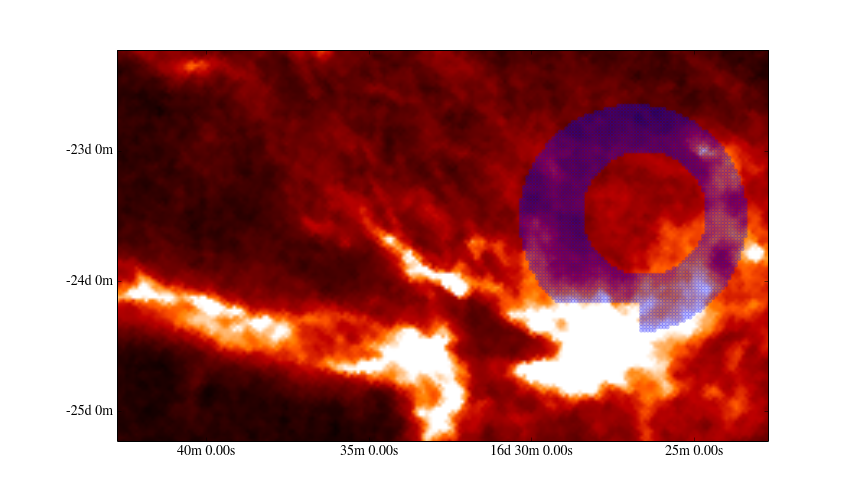
\includegraphics[scale=0.5]{fig/shell_2mass.png}
\caption{The shell region on top of the NICEST extinction map.
}
\end{figure*}

\subsubsection{The Cloud}
The mass within the cloud and the shell is estimated by calculating the mass within projected regions using the column density map. As discussed in \S4.1, we adopt the 2MASS extinction map in our mass calculation. We then calculate the mass column density from the equation (\citet{Arce_2001}):

\begin{equation}
\Sigma = \mu\,N_{H_2} = \mu\,(9.4\times10^{20})A_V\;\text{g/cm}^2
\end{equation}

$\mu$ is the average mass per particle and is $\sim$ 2.72 times mass of a hydrogen atom (a.m.u.) for molecular clouds in our Milky Way (ref?). We then obtain the total mass from $M = \Sigma\times \text{Area}$.

In the case of the Ophiuchus, we first calculate the threshold extinction value used to determine the edge of the cloud by calculating the average extinction in places with no obvious far-infrared emission. This threshold value is $\sim$ 0.93 mag. ($\sim$ $8.7 \times 10^{20}$ cm$^{-2}$) on our 2MASS extinction map. We then select the projected region of our cloud to include places where the extinction is larger than 0.93 mag. This threshold value is then subtracted from the extinction within the selected region. The total mass of the Ophiuchus cloud is estimated to be $\sim$ 6000 M$_{\sun}$.

The turbulent velocity of the cloud is estimated using the $^{12}$CO (1-0) line emission. Since the line profile in a molecular cloud at this scale varies from one part of the cloud to another, it is unsuitable to fit the profile and to calculate the velocity dispersion from the fit. A natural way to calculate the velocity dispersion is the second central moment:

\begin{equation}
\sigma_v = \sqrt{\left(\frac{\int{I(\mathbf{p}, v)\,(v(\mathbf{p}, v)-v_{cent}(\mathbf{p}))^2\,\text{d}(\mathbf{p}, v)}}{\int{I(\mathbf{p}, v)}\,\text{d}(\mathbf{p}, v)}\right)}\;\;\;\text{,}
\end{equation}

where $I(\mathbf{p}, v)$ and $v(\mathbf{p}, v)$ are the intensity and the velocity at each position $\mathbf{p}$ and velocity $v$, respectively. $v_{cent}(\mathbf{p})$ is the velocity centroid and is calculated from:

\begin{equation}
v_{cent} = \frac{\int{I(\mathbf{p}, v)\,v(\mathbf{p}, v)\,\text{d}(\mathbf{p}, v)}}{\int{I(\mathbf{p}, v)\,\text{d}(\mathbf{p}, v)}}
\end{equation}

This is also the first moment, which can be understood as the mean velocity weighted by the intensity at each velocity. In the data cube obtained at the FCRAO, the velocity resolution is 0.21 km/s, smaller than the typical thermal linewidth in molecular clouds ($\sim$ 1 km/s). Thus, we can use the discrete sum to calculate the integrals above without losing any information.

The average of the second central moment in the Ophiuchus cloud is $\sim$ 0.97 km/s. The rms velocity of the turbulence is $\sqrt{3}$ times the velocity dispersion and is thus $\sim$ 1.68 km/s on average over the cloud. To calculate the total momentum and energy in the turbulence, we match the maps of the second moment and the 2MASS/NICER extinction. We then calculate the momentum/energy within each pixel by using the extinction and the second moment at the pixel. For regions outside the coverage of the FCRAO observations, we adopt the mean second moment (0.97 km/s) for the turbulent velocity. Summing up the energy $E_i = 0.5\,M_i\,v_{turb,\,i}^2$ over the entire cloud gives us an estimate of the total momentum and energy in the turbulence. These are 9900 M$_{\sun}$ km/s and $8.82\times10^{46}$ erg, respectively.



\subsubsection{The Shell}
The ``bubble'' model (Silk 1985) of an embedded stellar wind predicts that we should observe a hot and relatively diffuse interior and a warm dense shell. In the case of the embedded stellar wind, the ``thickness'' of the shell is often much smaller than the radius of the shell (\citet{Churchwell_2007}; \citet{Arce_2011}), thus making the opacity of the shell smaller along lines of sight through the center of the shell. As a result, the projection of the shell on the sky often looks like a ``ring.'' Due to the variation of the density and the irregularity of the shape of the cloud, the ring is likely incomplete and asymmetric. Estimating mass from the column density within a projected area is thus a lower bound, and serves as a good proxy for the total mass of the shell when the shell is optically thin and symmetric. To estimate the mass of the shell, we first overlay the temperature and density maps to determine an elliptical region with a finite width in the warm and dense part of the map. Notice that we completely exclude the cluster region to avoid confusion between the gas in the shell and within the cluster (Fig. 14, on the 2MASS extinction map). After this projected region of the shell is determined, we use the 2MASS extinction map and convert the extinction magnitude into the mass column density using Eq. 11. Summing up the mass column density within the shell mass region then gives us the shell mass, estimated to be 462 $M_{\sun}$. This is a lower bound, since the cluster region we exclude when choosing the shell mass region likely contains gas within the shell.

The expanding velocity of the shell is determined from the average spectrum of the shell. The symmetry of the shell predicts that the velocity we observe with the molecular line emission within the ``ring'' is symmetric around some system velocity. That is, for each ``particle'' in the shell, the velocity is determined by ($v_{system}$ + $v_{expansion}\,\sin{\left(\cos^{-1}{\left(R/R_0\right)}\right)}$ + $v_{intrinsic}$), where $v_{intrinsic}$ is drawn from a velocity distribution characteristic of the molecule's intrinsic (microscopic) motion. Assuming that the line emission from $^{12}$CO (1-0) traces the gas component of the shell and that the intrinsic velocity distribution can be approximated by a normal distribution, we find $v_{expansion}$ from the residual of fitting the $^{12}$CO line with $N(v_{system}, \sigma)$. Fig. 15 shows the residual as well as the fitted Gaussian line profile, with an asymmetry of the residual due the opacity. $v_{residual}$ is $\sim$ 1.2 km/s, which is $v_{expansion}\,\sin{\left(\cos^{-1}{\left(R/R_0\right)}\right)}$ in the equation above. With the shell mass region selected to have an inner radius $\sim$ 0.98 pc and an outer radius $\sim$ 1.61 pc, we find $v_{expansion}$ to be $\sim$ 1.52 km/s. Notice that $v_{residual}$ is a lower bound since the residual calculated from the $^{12}$CO (1-0) line profile is likely probing the gas component at a larger radius than the inner radius due to the opacity effect.

From these estimates, we obtain the momentum and the kinetic energy of the shell. These are given by $P_{shell} = M_{shell}\,v_{expansion}$ and $E_{shell} = 0.5\,M_{shell}\,v^2_{expansion}$, respectively. For this shell, the momentum is $\sim$ 702 $M_{\sun}\,km/s$, and the energy is $\sim$ $1.06\times10^{46}\,erg$. This is $\sim$ 12 \% of the total turbulent energy of the cloud (compared to $\sim$ 15 \% for the largest shell in Perseus; Fig. 16). Notice again that since the estimates for the mass and the expansion velocity are both the lower limits of possible values, the momentum and energy of the shell presented here are likely smaller than the real values as well.

\begin{figure*}[ht]
\centering
%% The 'scale' parameter below allows you to scale the figure so that it fits within the page. In this case the figure was scaled to 20% of its original size. Note: for .png files one has to use pdflatex, not classic latex
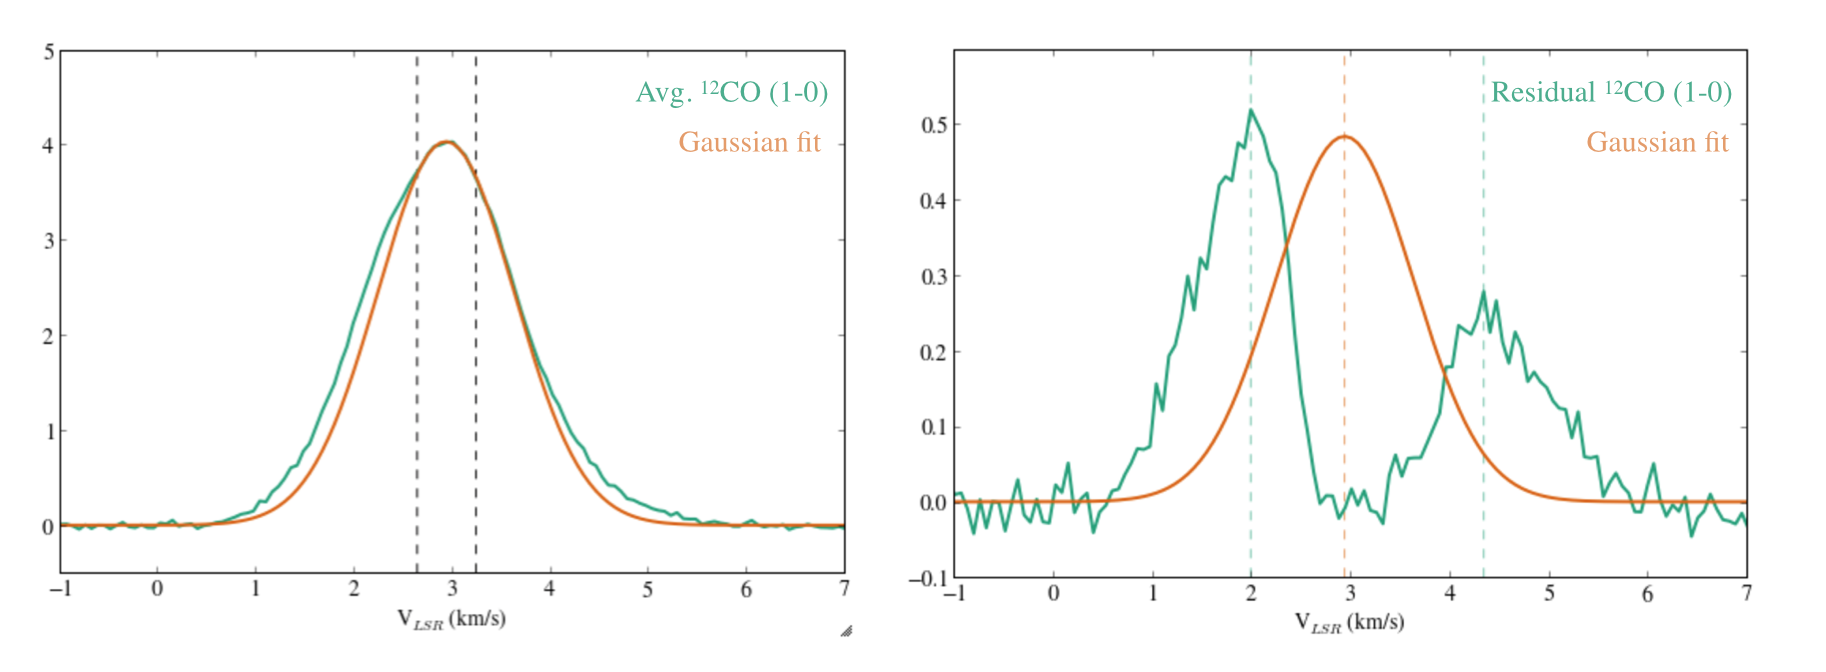
\includegraphics[scale=0.5]{fig/v_exp}
\caption{The expanding velocity of the shell, derived from FCRAO $^{12}CO$ data.
}
\end{figure*}

\begin{figure}[hb]
\centering
%% The 'scale' parameter below allows you to scale the figure so that it fits within the page. In this case the figure was scaled to 20% of its original size. Note: for .png files one has to use pdflatex, not classic latex
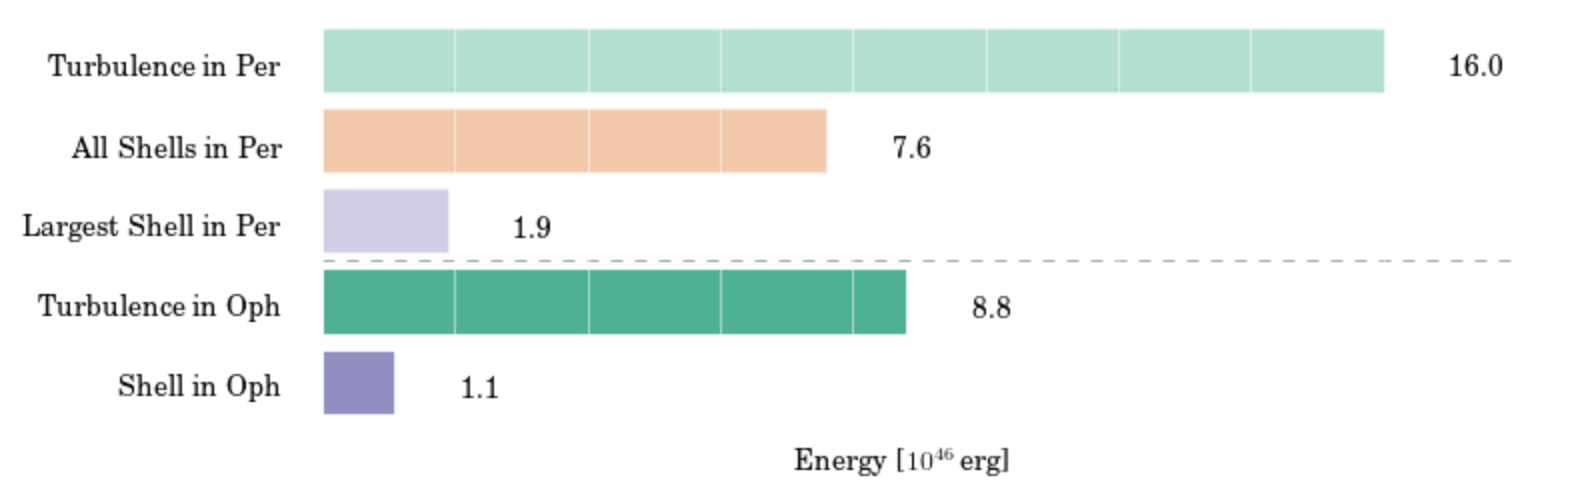
\includegraphics[scale=0.35]{fig/bar_energy.png}
\caption{Energy comparison between the shell and the clouds.
}
\end{figure}

\subsection{Impact of the Shell}
To estimate the impact of the shell on the cloud, we first compare the energy in the shell with the gravitational binding energy. With an effective radius of 5 pc (from the approximated geometrical mean of the cloud extent), we calculate the gravitational binding energy to be $3.97\times10^{47}$ erg, which is 30 times larger than the kinetic energy in the shell. Clearly, the shell does not have the energy to unbind the entire cloud.

One way to assess whether or not the embedded stellar wind is powerful enough to drive the turbulence is by comparing the energy injection rate ($\dot E_W$) of the shell to the turbulence dissipation rate ($L_{turb}$). The intuitive way to estimate the energy injection rate of the shell is to assume a timescale during which the wind from the embedded B-stars has been accumulating the kinetic energy that we observe within the shell. Following Arce et al. (2011), we assume $\tau_W$ $\sim$ $1\times10^6$ yr. We then have $\dot E_W = E_{shell}/\tau_W \sim 3.4\times10^{33}$ erg/s. Another way to assess this is following Eq. 3.7 in \citet{McKee_1989}:

\begin{equation}
\dot E_W = 0.5\,(\dot M_W\,v_W)\,v_{rms}\;\;\;\text{,}
\end{equation}

where $v_{rms}$ is the rms velocity of the turbulence in the cloud. $\dot M_W$ and $v_W$ are the mass loss rate and the wind velocity respectively. The mass loss rate of the shell can be estimated from the shell momentum we calculated in \S5.1 by assuming $\tau_W$ and a wind velocity $v_W$.

\begin{equation}
\dot M_W = \frac{P_{shell}}{\tau_W\,v_W}
\end{equation}

Assuming $\tau_W$ $\sim$ $6\times10^6$ yr and $v_W$ $\sim$ 200 km/s, we get a mass loss rate $\dot M_W$ $\sim$ $2.3\times10^{-5}$ M$_{\sun}$/yr. With the rms velocity of the turbulence $\sim$ 1.68 km/s, we get an energy injection rate of $\sim$ $10^{33}$ erg/s.

The turbulence dissipation rate depends on the dissipation time, which is related to the free-fall time and is often written as $t_{diss} = \eta\,t_{ff}$. In \citet{McKee_1989} and McLow (1999), numerical simulations give $\eta$ in the range of 1 to 10. Assuming $\eta$ = 5 and a volume density of $10^3$ cm$^{-3}$, we have $t_{diss}$ $\sim$ $5\times10^6$ yr. We can then calculate the turbulence dissipation rate:

\begin{equation}
L_{turb} = \frac{E_{turb}}{t_{diss}}
\end{equation}

This gives $L_{turb}$ $\sim$ $10^{33}$ erg/s, which is on the same order of magnitude as the energy injection rate of the shell. These estimates indicate that the spherical wind from B-stars ($\rho$ Oph) has the potential for driving the turbulence in the Ophiuchus cloud. This result agrees with \citet{Arce_2011}.

\begin{table*}
\centering
\begin{tabular}{lcc}
\hline
& \textbf{Shell in Ophiuchus} & \textbf{CPS5 in Perseus} \\   
\hline
Radius (IR) [pc] & 1.30 & 2.65 \\ 
Mass [M$_{\odot}$] & 462 & 53 \\ 
Expansion Velocity [km/s] & 1.2 & 3 \\ 
Momentum [M$_{\odot}$ km/s]& 702 & 315 \\ 
Kinetic Energy [erg]& 1.06$\times10^{46}$ & 1.88$\times10^{46}$ \\ 
... of total turbulent energy & (12.0\%) & (11.8\%) \\ 
Energy Injection Rate [erg/s] & 2.46$\times10^{33}$ & 1.49$\times10^{32}$ \\
\hline
\end{tabular}
\caption{Comparison between the shell in Ophiuchus and the shell with the largest radius, CPS5, in Perseus (Arce et al 2011)}
\end{table*}

\subsection{Comparing to Perseus}
Table 1 shows the physical properties of the shell discussed here and the largest shell (CPS 5) in the Perseus (\citet{Arce_2011}). We find that while the momenta of the two shells are comparable, the shell in the Ophiuchus cloud is more massive with a lower expansion velocity. This results in its smaller kinetic energy. However, since the total energy in the turbulence is smaller in the Ophiuchus cloud, the ratios of the shell energy to the turbulence energy in the cloud are comparable to each other. In the comparison of the energy injection rate and the turbulence dissipation rate, the shell in the Ophiuchus is powerful enough to drive the turbulence by itself, while in the Perseus, all shells with confidence scores larger than 4 (\citet{Arce_2011}) are required to get an energy injection rate at the same order of magnitude as the turbulence dissipation rate. We think that this hints at the fundamental difference between the two clouds and the shell(s) therein. The Ophiuchus cloud is slightly smaller than the Perseus cloud in terms of its mass and size, and the larger mass/smaller velocity of the shell in the Ophiuchus cloud probably indicates that the shell has been expanding for a longer period of time.


\section{Discussion}
\label{sec:discussion}

\subsection{Column density tracers: when to use what}

\subsection{Shell-like structure: an embedded B-star wind?}

\subsection{(Non-)Correlation between column density distribution and the dynamics in a molecular cloud}

\section{Conclusions}
In this work, multi-wavelength observations enable us to analyse the derivation of physical properties in the interstellar medium. By doing this, we provide a reliable estimate of the energy and momentum in the cloud and the shell-like structure of an embedded B-star wind. We find that, although this one shell is not powerful enough to sustain the turbulence in the entire cloud, it does inject a substantial amount of energy into the cloud. Here we list our conclusions:

\begin{itemize}
\item Three of the most common ways to trace the column density in molecular clouds include the near-infrared extinction, mid/far-infrared thermal emission and molecular line emission. Comparing the results using data from 2MASS, IRIS, Herschel and FCRAO, we find that the 2MASS/NICER-based extinction measurement serves as the most reliable tracer of column densities in the cloud. However, each of these different tracers, including the 2MASS/NICER-based extinction, suffers from its own limits. This is because none of these tracers directly trace the most dominant component of mass in molecular clouds: the molecular hydrogen. The variation of dust-to-gas ratio and the dust properties affect the effectiveness of both dust tracers, while the excitation criterion (for example, the critical density and temperature) makes it difficult to assess the conversion from the line emission to the gas column density. In dense regions, the molecular line emission can be optically thick or depleted, making it unsuitable for tracing the column density. Following \citet{Goodman_2009}, we propose that when choosing tracers of the column density, one should always consider the physical environment of the target region. 
\item Two of the complexities of using the mid/far-infrared emission as a density tracer are the variation of physical properties along the line of sight and the noise in the data. The commonly used modified blackbody equation assumes a single temperature, column density and the emissivity spectral index $\beta$ throughout the entire line of sight. This makes it difficult to describe the observed SED with the modified blackbody equation, especially when we free both the temperature and $\beta$ in the fitting. By building a toy line of sight, we find that the temperature and $\beta$ derived by fitting the modified blackbody equation are not representative of a line of sight with a varying temperature and $\beta$. On the other hand, we experiment with the hierarchical Bayesian-fitting method in the hope of decreasing the bias caused by noise in the data. We find that while it decreases the bias we see in previous works, including the anti-correlation between the temperature and $\beta$, the original code used in \citet{Kelly_2012} is not readily applicable to extended sources. To build a hierarchical Bayesian-fitting method that treats the distributions in the parameter space and of the observed fluxes at the same time, we need a more sophisticated model for these distributions than the multivariate Student-T distribution used in \citet{Kelly_2012}.
\item With a better understanding of various density tracers, we calculate the total turbulent energy in the Ophiuchus cloud and the energy entrained in the embedded B-star wind. By comparing the two, we find that the energy in the shell strucuture caused by the B-star wind amounts to $\sim$ 12 \% of the total turbulent energy in the cloud. The wind's energy injection rate is also comparable to the dissipation rate of the turbulent energy in the entire cloud. Comparing this result to shells in the Perseus cloud (Arce et al. 2011), we find that the shell in the Ophiuchus has energy comparable to the largest few shells in the Perseus and its energy injection rate is comparable to the \emph{sum} of all shells in the Perseus. We conclude that the embedded stellar winds can contribute to the turbulent energy in molecular clouds. In future simulations, embedded winds driven by B or even later types of stars should be included as important sources of turbulence in molecular clouds.
\end{itemize}



%\bibliography{bibliography/converted_to_latex.bib%
%}

\bibliographystyle{apj}
\bibliography{oph_shell}

\end{document}
